\chapter{Estimating Zipf's Law parameters} \label{zr}

\citet{Zipf1949} notes that word frequencies show a sparse distribution. \citeauthor{Zipf1949} notes a linear relationship between log word frequency $r$ and log frequency $r$. A generalized form of this relationship is what is now known as Zipf's Law.

\begin{unlabeledexample} 
$\displaystyle f(C, \alpha) = \frac{C}{r^\alpha}$ 
\end{unlabeledexample} 

\noindent $C$ is a constant which is primarily sensitive to sample size. \citeauthor{Zipf1949}'s assumes that $\alpha = -1$, but both $C$ and $\alpha$ can be estimated using the method of least squares ($\epsilon$ represents the error term).
 
\begin{unlabeledexample} 
$\displaystyle \textrm{log}~f \sim C + \alpha~\textrm{log}~r + \epsilon$  
\end{unlabeledexample}

\citet{Good1953} notes that sparse empirically-estimated distributions exhibit quantization at low frequencies, producing an artificially long and flat right tail and biasing $\alpha$ upward. \citet[][29]{Church1991} describe a transform to eliminate this quantization. The vectors $r, n$ are defined so such that $n_i$ is the number of types which occur at frequency $r_i$ (that is, $n$ is a vector of frequencies of individual type frequencies). $Z$ is simply a vector in which each element of $n$ scaled by the nearest points to the left and right.

\begin{unlabeledexample}
$\displaystyle Z_i = \frac{2 n_i}{r_{i + 1} - r_{i - 1}}$
\end{unlabeledexample}

\noindent \citeauthor{Church1991} do not define this transform for the lowest and highest points (i.e., when $i = 1$ or $i = N$), but a natural extension of their definition is to scale the endpoints according to the next intermost point, as defined below.

\begin{unlabeledexample}
$\displaystyle Z_1 = \frac{n_1}{r_2 - r_1}$
\end{unlabeledexample}

\begin{unlabeledexample}
$\displaystyle Z_N = \frac{n_N}{r_N - r_{N - 1}}$
\end{unlabeledexample}

\noindent The effect of applying this transform to sparse frequency data is shown in Figure \ref{subtlex}.

\begin{figure}
\centering
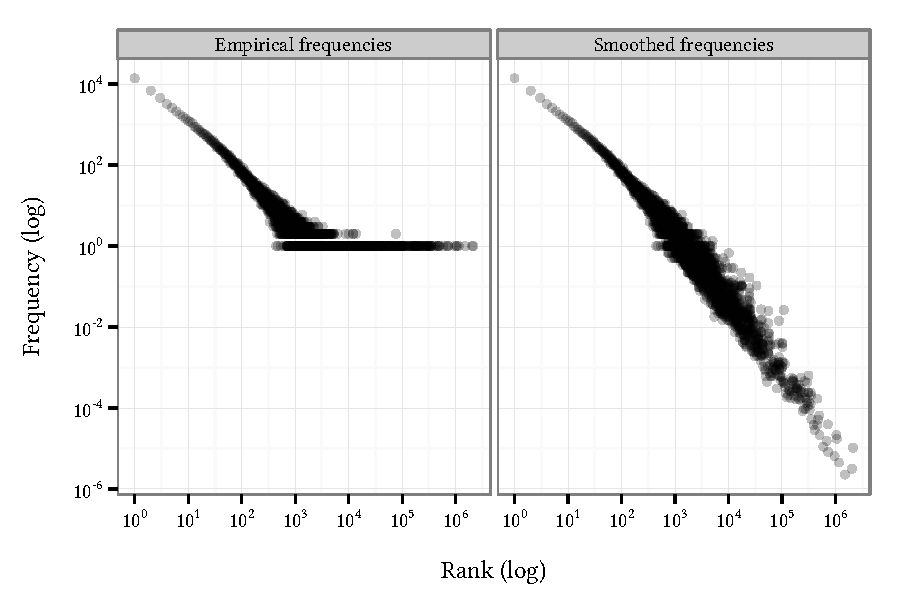
\includegraphics{zr.pdf}
\caption{The left panel shows the empirical word frequencies in SUBTLEX-US \citep{Brysbaert2009}. The right panel shows the effect of the $Z_r$ transform.}
\label{subtlex}
\end{figure}
